\selectlanguage{ngerman} %ngerman or english      
\title{\textbf{Bericht}\break \\ 24FS\_I4DS27: Adversarial Attacks \\ Wie kann KI überlistet werden?} 

\begin{titlepage}
    \textcolor{white}{Easteregg: Team Secondos}
    \vfill
    \centering
    \vspace{0.5cm}
    \huge{\textbf{Bachelor Thesis}}
    
    \vspace{0.1cm}
    \huge{24FS\_I4DS27: Adversarial Attacks \\ Wie kann KI überlistet werden?}
    \vspace{0.1cm}
    
    \Large{Windisch, \germandate\today}      

    \begin{figure}[H]
        \centering
        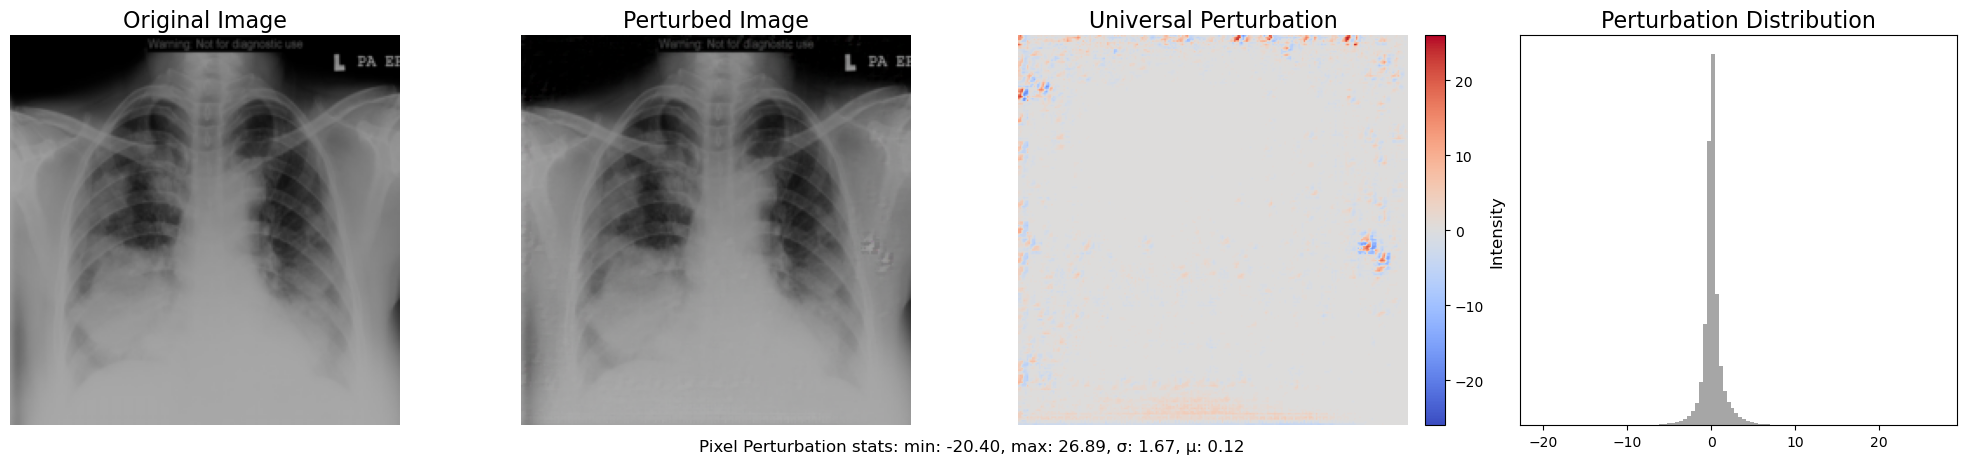
\includegraphics[width=0.8\columnwidth]{01-images/01-setup/01-titleimage.png}
    \end{figure}
    
    \large{
    \begin{tabular}{@{}p{7.0cm}l}
        Studenten                  &    Si Ben Tran\\
                                   &    Gabriel Torres Gamez\\[2ex]
        
        Fachbetreuer               &    Daniel Perruchoud\\
                                   &    Stephan Heule\\[2ex]
                                   
        Auftraggeber               &    i4Ds\\
        Projektnummer              &    24FS\_I4DS\\[4ex]
        
        \multicolumn{2}{@{}l}{Fachhochschule Nordwestschweiz, Hochschule für Technik}
    \end{tabular}
    }
    
    \begin{tikzpicture}[remember picture,overlay,every node/.style={anchor=north east}]
      \node at (current page.north east) [xshift=-1cm, yshift=-0.4cm] {
\includegraphics[width=4cm]{01-images/01-setup/02-logo.png}};
    \end{tikzpicture}
    
    \begin{tikzpicture}[remember picture,overlay,every node/.style={anchor=north west}]
      \node at (current page.north west) [xshift=1cm, yshift=-1.2cm] {
\includegraphics[width=9cm]{01-images/01-setup/03-fhnwlogo.pdf}};
    \end{tikzpicture}
    
    \clearpage
    
\end{titlepage}